
\subsection{General Game Playing}

Most research in artificial intelligence (AI) game-playing has focused on developing programs that can play one
game at a strong level. These programs 
generally rely on human-expert knowledge embedded into the programs by the software developers. In General Game Playing 
(GGP)~\cite{Genesereth05GGP} the aim is to create programs that can learn to play a wide variety of games. 
GGP engines are given as input only the game's description, with
human intervention disallowed, so no prior domain-specific knowledge can be incorporated ahead of time.

Games rules are described using the Game Description Language~\cite{Love08GDL}. In GDL, at every state each player has 
a set of available actions and transitions from state to state require that all players submit a legal action. In essence, 
every game is described as a simultaneous move game, but strictly sequential games can be modeled by, at every state, 
having the a single player with possibly many legal moves with that player's opponents restricted to a single legal 
\textit{no-op} move. 
 
General game playing is a field of AI that encourages the development of general artificial intelligence, and as such
has generated much interest among researchers. 
Since 2005, nine yearly GGP competitions have taken place and three academic workshops have focused on GGP. 
Several web sites have been created to maintain software and host repositories of game descriptions, and 
a massively open online course was given in 2013. This year's competition is set for summer of 2014. 

% Seems to be done later in the experiments section.. ?
%\mlanctot{Mention that we're not using GDL and why?}

\mlanctot{@Mandy: can you add the $C$ parameter below in the appropriate place? (I'm not sure where you put it.)}

%
%% DUCB1T
%

An enhancement to the UCT selection strategy can be made by replacing the parameter $C$ by an upper bound of the variance of 
the rewards. This is either $\frac{1}{4}$, which is an upper bound of the variance of a $\{0,1\}$-outcome Bernoulli
random variable, or an upper confidence bound computed using Equation~\ref{ucb1tuned}. 
This variant is referred to as UCB1-Tuned~\cite{Auer02Finite}. Then, an action is selected from parent 
node $s$ using:

\begin{equation}
\label{ucb1tuned}
a^* = \argmax_{a \in \cA(s)} \left\{ \bar{X}_{s,a} + C \times \sqrt{\frac{\min(\frac{1}{4},\mathrm{Var}_{\mathit{UCB1}}(s,a)) \ln (n_{s})}{n_{s,a}}} \right\}, 
\end{equation}
\[
\mbox{Var}_{\mathit{UCB1}}(s,a)=\mbox{sv}^2_{s,a}\sqrt{\frac{2 \ln (n_{s})}{n_{s,a}}},
\]
where $\mbox{sv}^2_{s,a}$ is the sample variance of the observed rewards for taking action $a$ from $s$. 
When UCB1-Tunded is used in the tree setting, we refer to it as the SM-MCTS variant {\it Decoupled UCB1-Tuned}, or DUCB1T for short.

\begin{table}[h]
\caption{Parameters}
\label{table:parameters}
\centering
\begin{tabular}{|c|c|c|c|c|c|}
\hline
  & DUCT & DUCB1T & SUCT & Exp3 & RM  \\
\hline
Battle            & $C=0.0$ & $C=0.0$ & $C=0.4$ & $\gamma = 0.8$ & $\gamma = 0.10$  \\ 
BiddingTicTacToe  & $C=0.0$ & $C=0.0$ & $C=0.0$ & $\gamma = 0.9$ & $\gamma = 0.15$   \\ 
Chinook           & $C=0.4$ & $C=0.4$ & $C=0.4$ & $\gamma = 0.2$ & $\gamma = 0.30$ \\ 
Goofspiel         & $C=0.4$ & $C=0.4$ & $C=0.8$ & $\gamma = 0.1$ & $\gamma = 0.20$ \\ 
Oshi-Zumo         & $C=0.4$ & $C=0.4$ & $C=1.8$ & $\gamma = 0.6$ & $\gamma = 0.75$ \\ 
PawnWhopping      & $C=0.0$ & $C=0.4$ & $C=0.4$ & $\gamma = 0.4$ & $\gamma = 0.75$  \\ 
RacetrackCorridor & $C=1.2$ & $C=0.8$ & $C=0.8$ & $\gamma = 0.4$ & $\gamma = 0.15$\\ 
Runners           & $C=0.8$ & $C=0.4$ & $C=1.8$ & $\gamma = 0.3$ & $\gamma = 0.50$ \\
Tron              & $C=1.8$ & $C=2.0$ & $C=2.0$ & $\gamma = 0.3$ & $\gamma = 0.30$ \\
 \hline
\end{tabular}
\end{table}


\begin{figure*}[h!]
\centering
\begin{subfigure}{9cm}
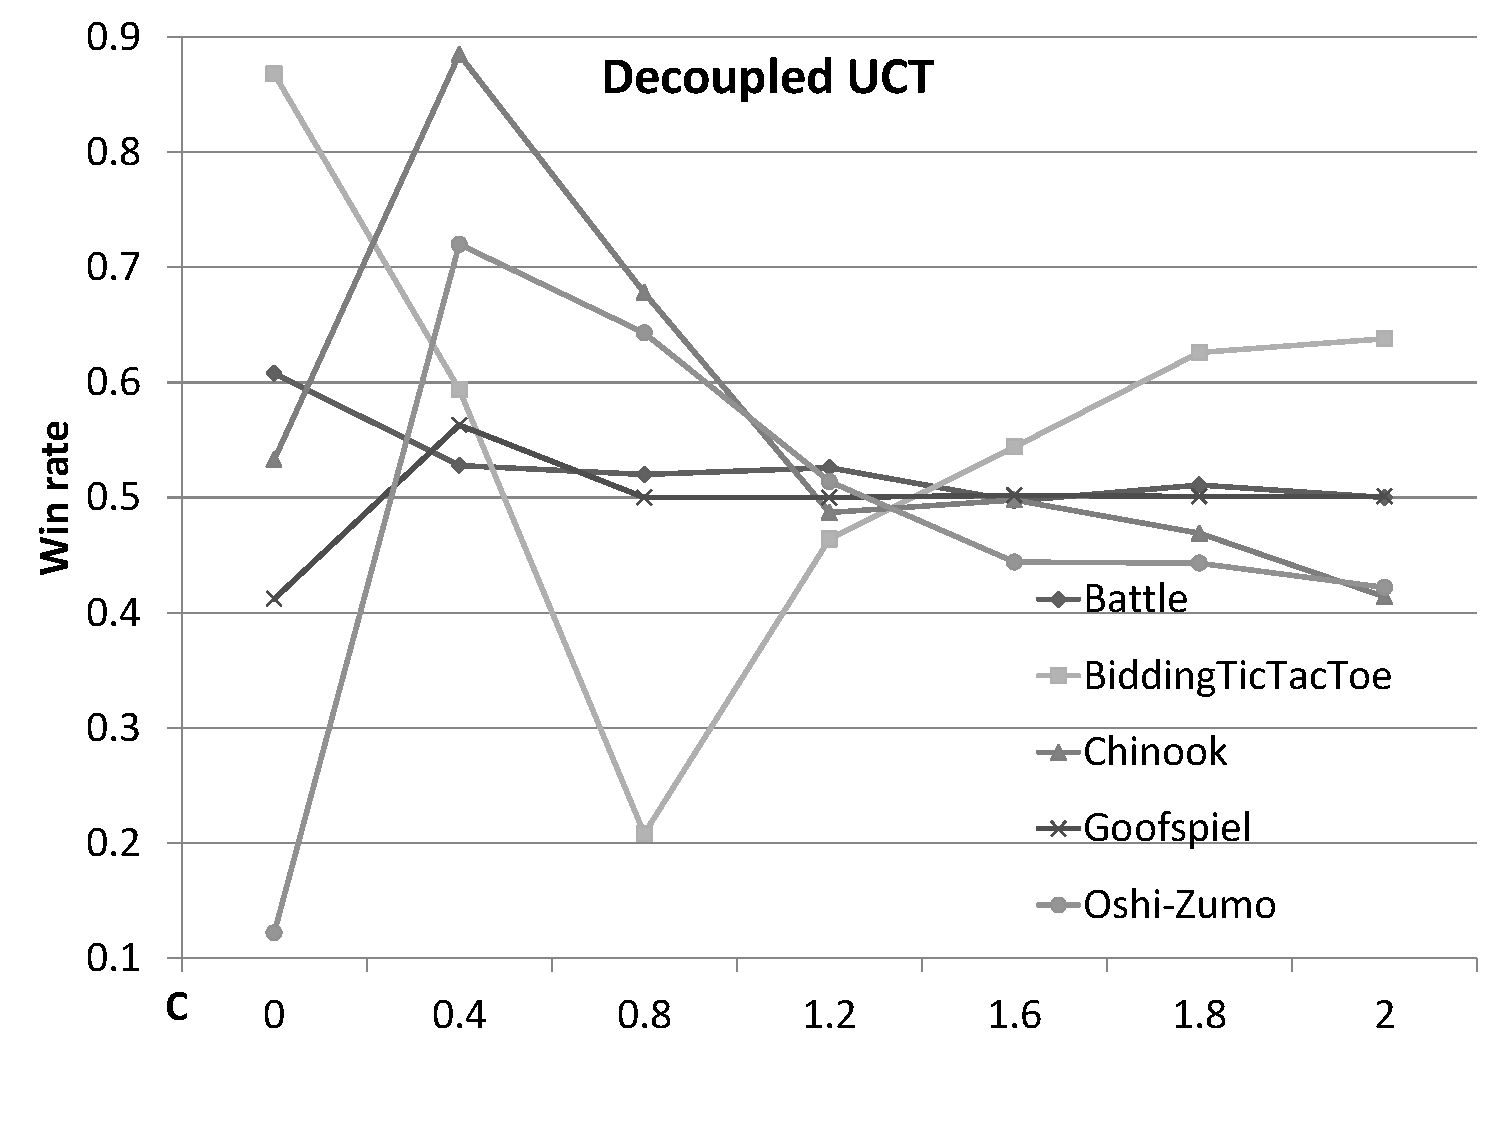
\includegraphics[width=8.0cm]{figures/duct1}\\
\end{subfigure}
\begin{subfigure}{9cm}
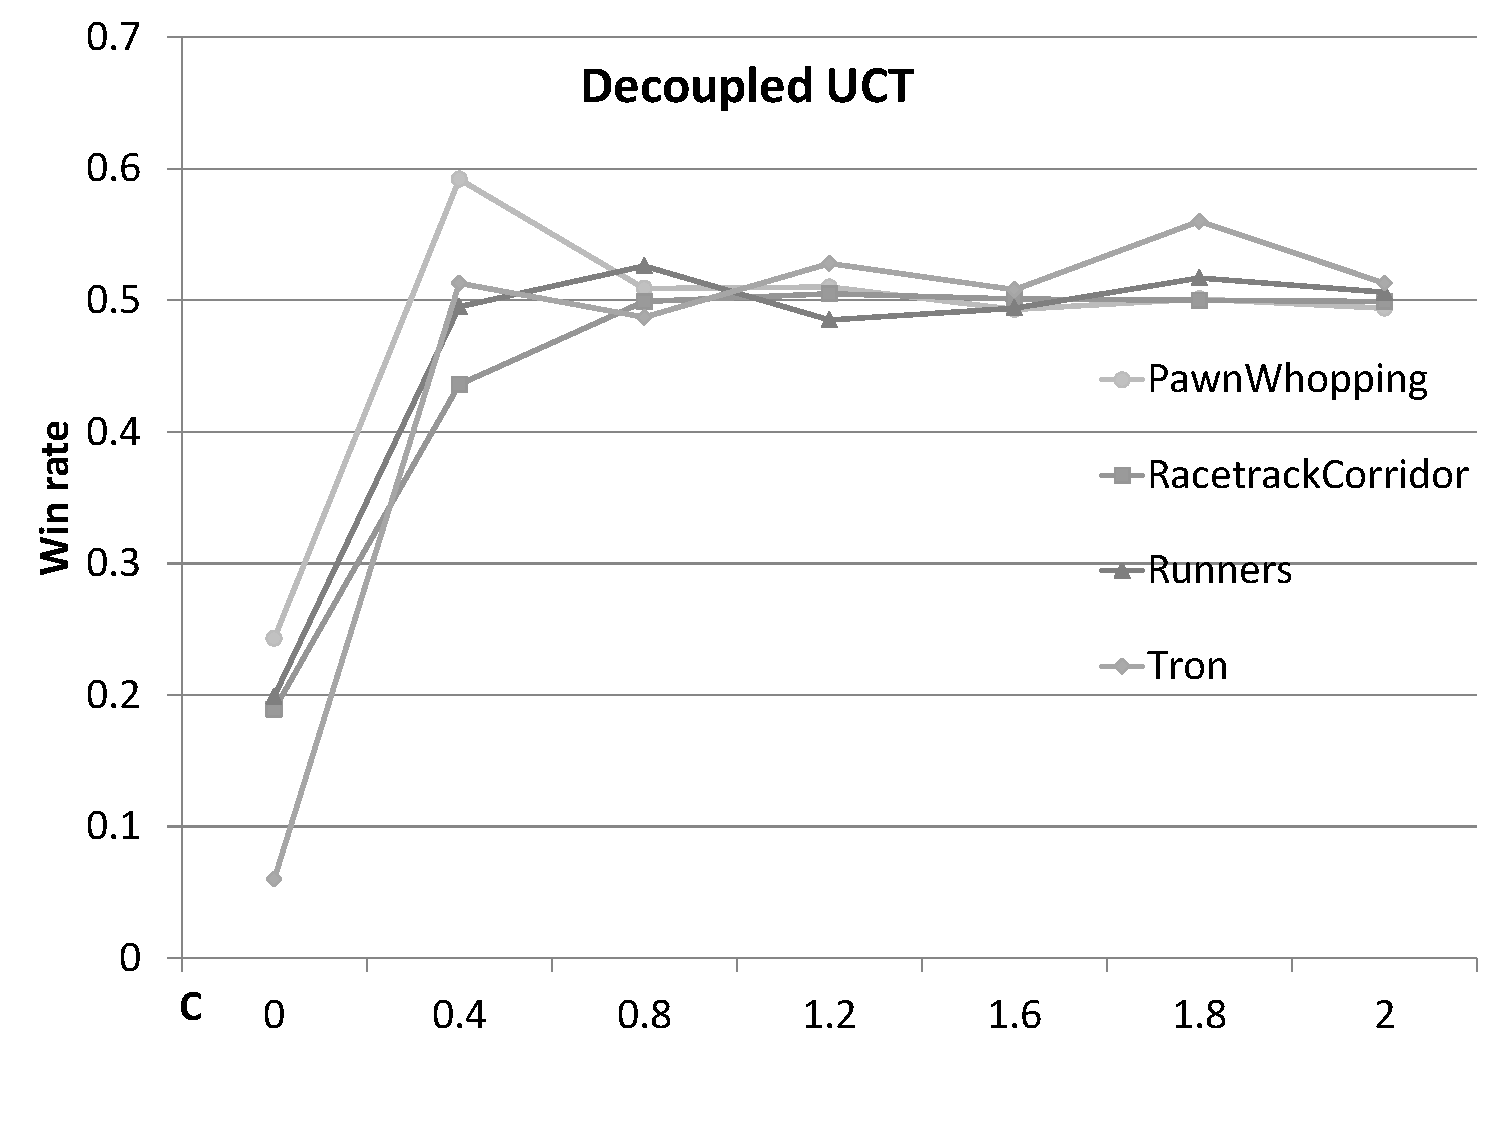
\includegraphics[width=8.0cm]{figures/duct2}\\
\end{subfigure}
\begin{subfigure}{9cm}
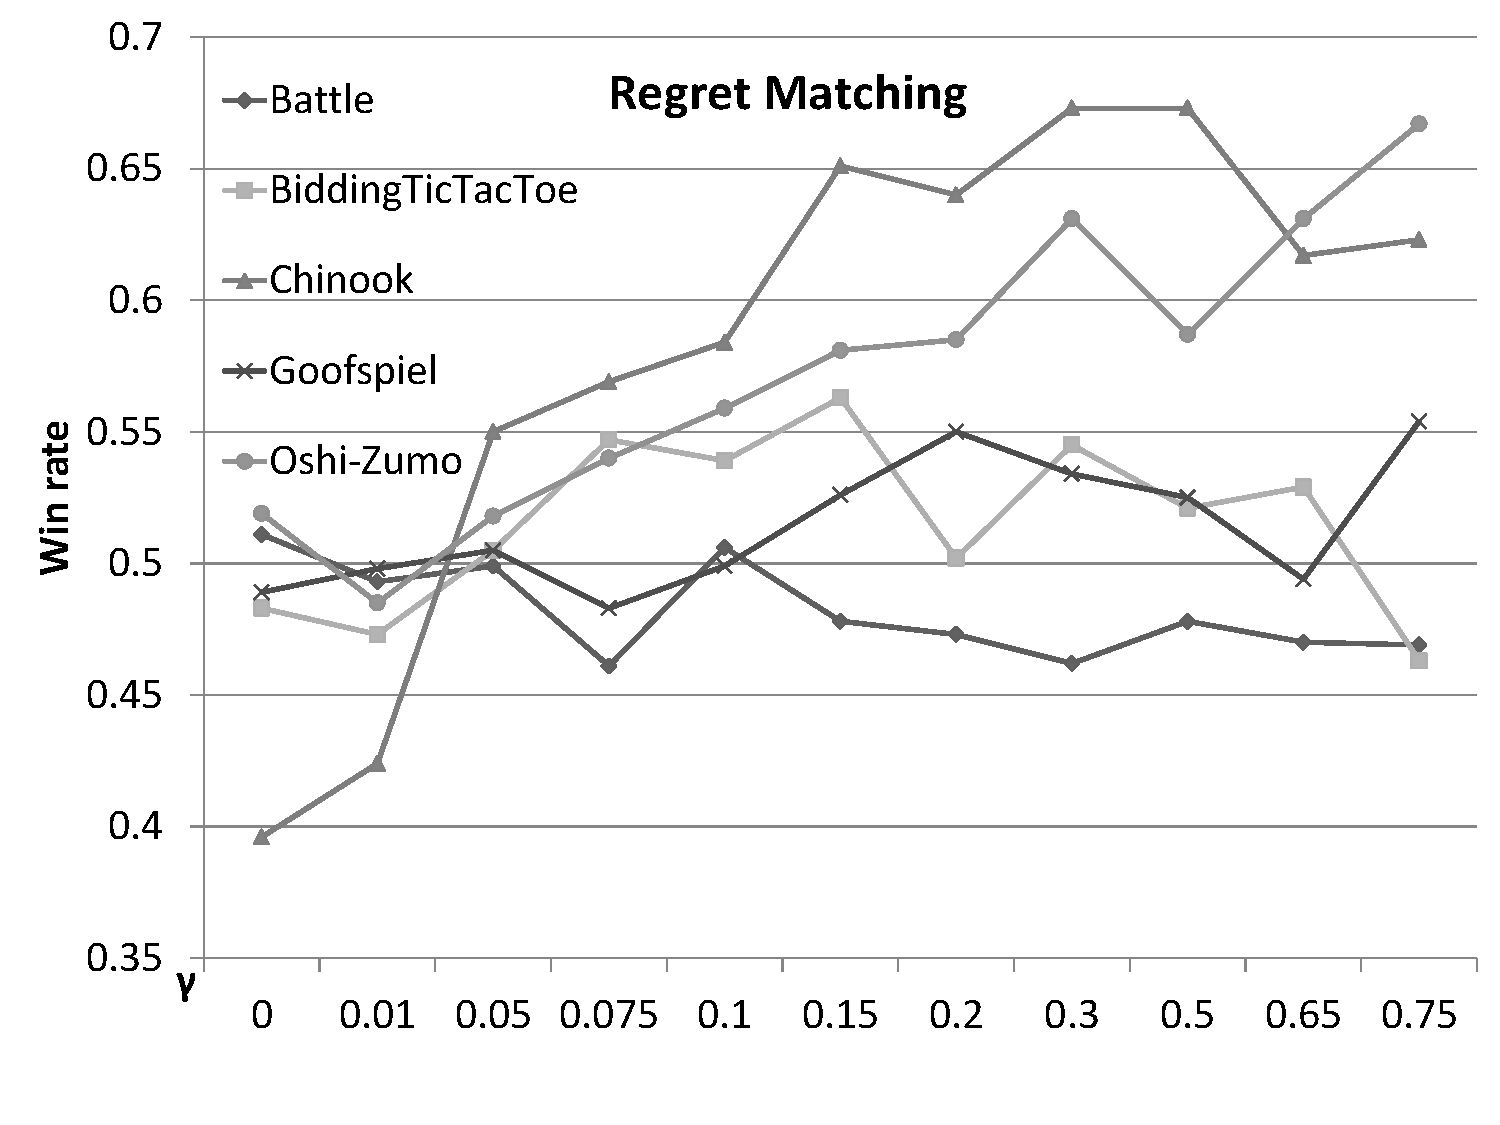
\includegraphics[width=8.0cm]{figures/regretmatching1}\\
\end{subfigure}
\begin{subfigure}{9cm}
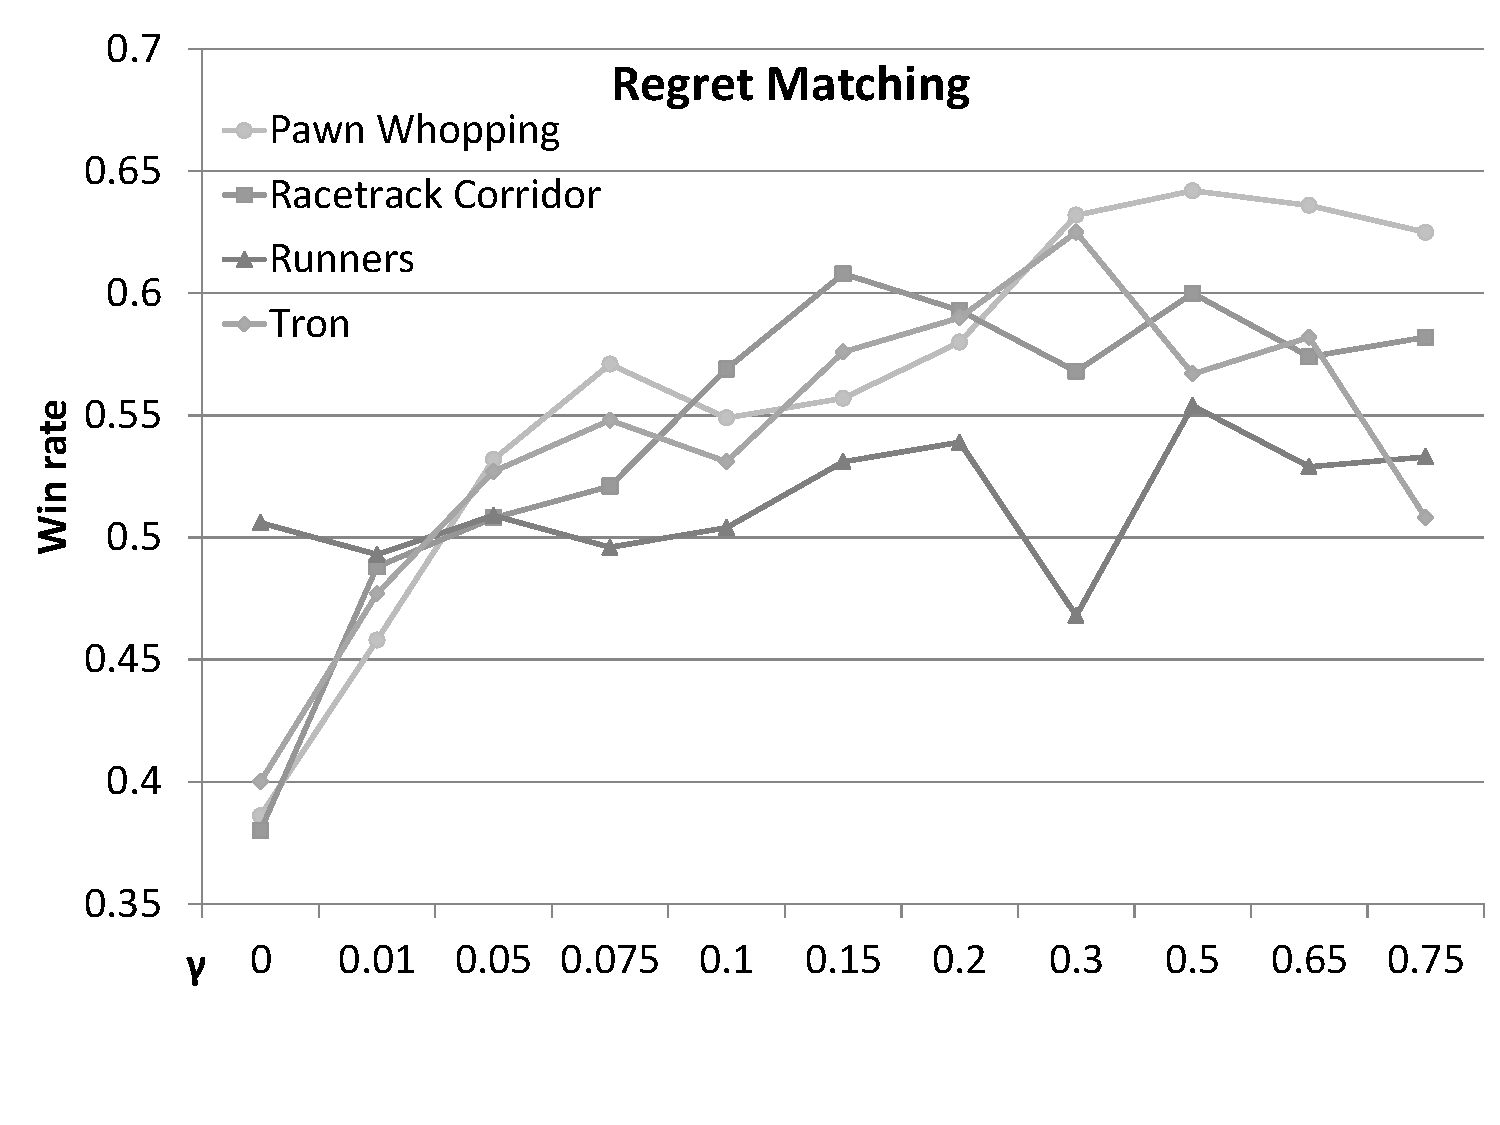
\includegraphics[width=8.0cm]{figures/regretmatching2}\\
\end{subfigure}
\caption{Tuning Regret Matching and Decoupled UCT}
\label{fig:tuning1}
\end{figure*}



